\documentclass[10pt,a4paper]{article}
\usepackage{pgfplots}
\pgfplotsset{compat=newest}
\pgfplotsset{
	integral segments/.code={\pgfmathsetmacro\integralsegments{#1}},
	integral segments=3,
	integral samples/.code={\edef\integralsamples{#1}},
	integral samples = 10,
	integral min/.style args={#1:#2}{
		ybar interval,
		domain=#1:#2,
		samples=\integralsegments+1,
		x filter/.code={
			\edef\lastx{\pgfmathresult}
			\pgfmathresult
		},%
		y filter/.code={%
			\pgfmathparse{(#2/(\integralsegments))/\integralsamples}%
			\edef\tempstep{\pgfmathresult}%
			\pgfmathparse{f(\lastx)}%
			\edef\tempa{\pgfmathresult}%
			\edef\tempb{\pgfmathresult}%
			\foreach \x in {0,1,...,\integralsamples}%
			{%
				\pgfmathparse{f(\lastx+\x*\tempstep)}%
				\xdef\tempb{\tempb,\pgfmathresult}%
			}%
			\pgfmathmin{\tempb}{\tempb}
		},
	},
	integral max/.style args={#1:#2}{
		ybar interval,
		domain=#1:#2,
		samples=\integralsegments+1,
		x filter/.code={
			\edef\lastx{\pgfmathresult}
			\pgfmathresult
		},%
		y filter/.code={%
			\pgfmathparse{(#2/(\integralsegments))/\integralsamples}%
			\edef\tempstep{\pgfmathresult}%
			\pgfmathparse{f(\lastx)}%
			\edef\tempa{\pgfmathresult}%
			\edef\tempb{\pgfmathresult}%
			\foreach \x in {0,1,...,\integralsamples}%
			{%
				\pgfmathparse{f(\lastx+\x*\tempstep)}%
				\xdef\tempb{\tempb,\pgfmathresult}%
			}%
			\pgfmathmax{\tempb}{\tempb}
		},
	},   
}
\makeatletter
%see https://tex.stackexchange.com/questions/9722/why-am-i-getting-the-pgf-math-error-unknown-function-getargs
\def\pgfmathmax#1#2{%
	%   \pgfmathparse{getargs(#1,#2)}%
	\pgfmathparse{#1,#2}%
	\expandafter\pgfmathmax@\expandafter{\pgfmathresult}%
}
\def\pgfmathmin#1#2{%
	\pgfmathparse{#1,#2}%
	\expandafter\pgfmathmin@\expandafter{\pgfmathresult}%
}
%see https://tex.stackexchange.com/questions/15435/how-do-i-use-pgfmathdeclarefunction-to-create-define-a-new-pgf-function
\makeatother
\begin{document}
	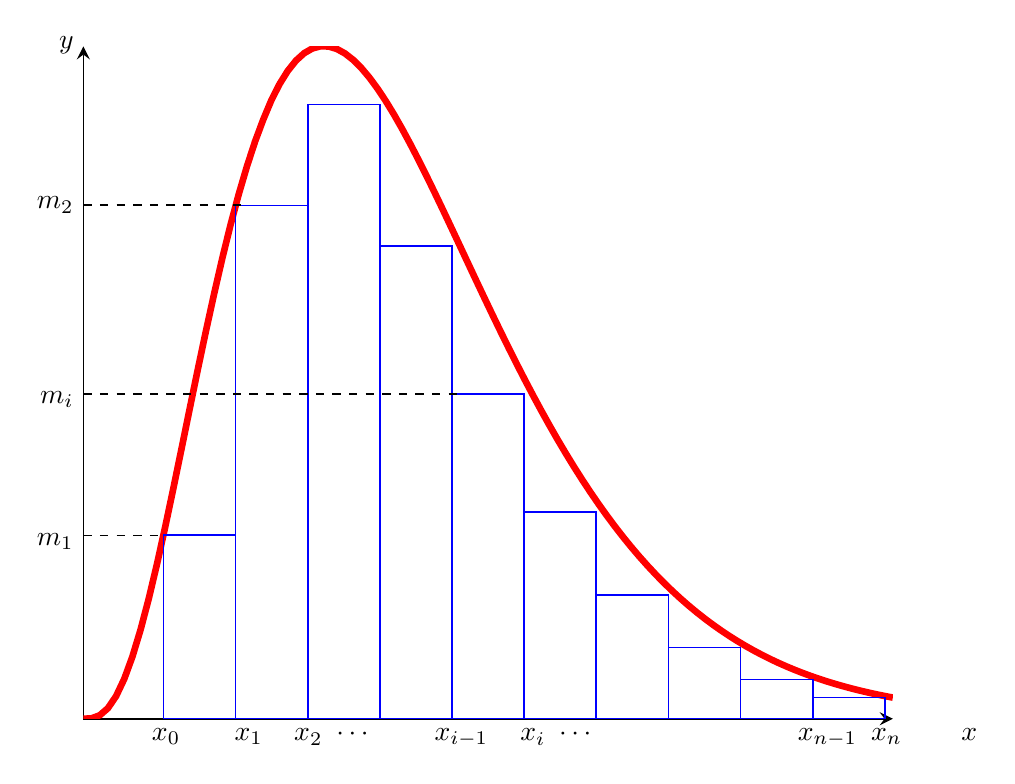
\begin{tikzpicture}[scale=1.5]
		\pgfset{declare function={f(\x)=3*exp(-(\x))*(\x)^3+1;}}
		\begin{axis}[ticks=none,
			domain=0:10.1,
			samples=100,
			axis lines=middle,
			xticklabels={},
			yticklabels={}
			]
			\addplot [ultra thick,red] {f(x)};
			
			\addplot [blue,
			integral segments=10,
			integral min=1:10
			] {f(x)};
		\end{axis}
	
	\node[below] at (.7,0) {$x_0$};
	\node[left] at (0,1.5) {$m_1$};
	\draw[dashed] (0,1.55) -- (.7,1.55);
	
	\node[below] at (1.4,0) {$x_1$};
	\node[left] at (0,4.35) {$m_2$};
    \draw[dashed] (0,4.35) -- (1.4,4.35);
    \node[below] at (2.1,0) {$x_2\ \cdots$};
	
	
	\node[below] at (3.2,0) {$x_{i-1}$};
	\node[below] at (4,0) {$x_{i}\ \cdots$};
	\node[left] at (0,2.7) {$m_i$};
    \draw[dashed] (0,2.75) -- (3.2,2.75);
    
    \node[below] at (7.5,0) {$x$};
    \node[left] at (0,5.7) {$y$};
    
   	\node[below] at (6.8,0) {$x_{n}$};
  	\node[below] at (6.3,0) {$x_{n-1}$};
	
	\end{tikzpicture}
	\hfill
	
	
	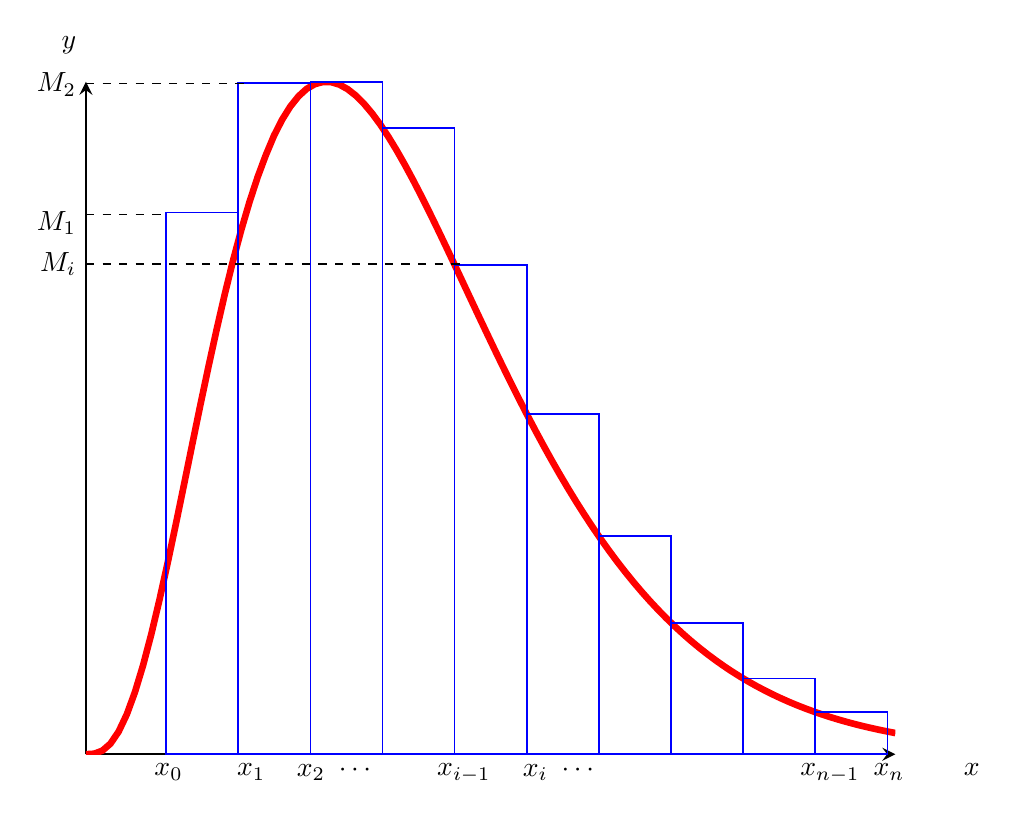
\begin{tikzpicture}[scale=1.5]
		\pgfset{declare function={f(\x)=3*exp(-(\x))*(\x)^3+1;}}
		\begin{axis}[ticks=none,
			domain=0:10.1,
			samples=100,
			axis lines=middle
			]
			\addplot [ultra thick,red] {f(x)};
			
			\addplot [
			blue,
			integral segments=10,
			integral max=1:10
			] {f(x)};
		\end{axis}
	
		\node[below] at (.7,0) {$x_0$};
	\node[left] at (0,4.5) {$M_1$};
	\draw[dashed] (0,4.57) -- (.7,4.57);
	
	\node[below] at (1.4,0) {$x_1$};
	\node[left] at (0,5.67) {$M_2$};
	\draw[dashed] (0,5.68) -- (1.4,5.68);
	\node[below] at (2.1,0) {$x_2\ \cdots$};
	
	
	\node[below] at (3.2,0) {$x_{i-1}$};
	\node[below] at (4.,0) {$x_{i}\ \cdots$};
	\node[left] at (0,4.15) {$M_i$};
	\draw[dashed] (0,4.15) -- (3.2,4.15);
	
	\node[below] at (7.5,0) {$x$};
	\node[left] at (0,6) {$y$};
	
	\node[below] at (6.8,0) {$x_{n}$};
	\node[below] at (6.3,0) {$x_{n-1}$};
	
	
	\end{tikzpicture}
	
	
	
	
\end{document}
